\section{Choosing a vision on the loop solution}

In order to create our embedded system, we have to follow somme specifications : 

\begin{enumerate}
 \item The system is composed by a camera mounted on two servomotors (JIWY2) and controlled by one of this setup :
 \begin{enumerate}
  \item Combination of an altera DE0-NANO and an Overo fire.
  \item RaMstix extension board for Overo FireStorm-P
 \end{enumerate}
 \item The system is able to process image form the camera and move the camera in fonction.
\end{enumerate}

In order to follow this specifications, there is several option. For example, we could have created a system that goes alternatively to differents colors or try to avoid capting a specific shape. This systems although funnier to create and use would have been more difficult to implement therefore we finally chose and easier system that consist on following a specific color shape on the picture get by the webcam to have this shape in the center of thhe picture.

\begin{figure}[!ht]
\centering
 \includegraphics[width=0.5\textwidth]{visionOnTheLoop.png}
 \caption{Our vision-on-the-loop solution}
 \label{votl}
\end{figure}

\section{Units definition}

The first step to design such a system is  to define all the functional units we need. Each functional unit will also be divided in subsystems untill we get an easy enough unit to implement it. In our case, we can define 4 units of first level : 

\begin{itemize}
 \item An encoder block that give a feedback about the position of the camera
 \item A PWM block that control the the camera movement
 \item An image processing block which take picture frome the camera and get the position of the object we want to detect,
 \item A control loop that translate feedback to order
\end{itemize}

\begin{figure}[!ht]
\centering
 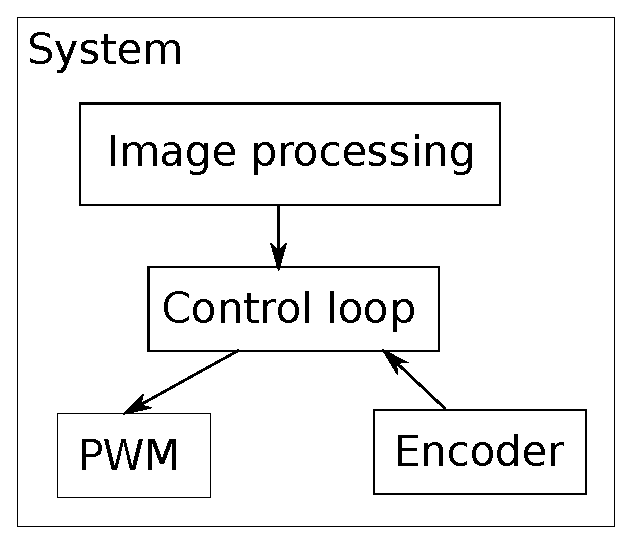
\includegraphics[width=0.5\textwidth]{dessin-1.eps}
 \caption{Sytem schematic : first level}
 \label{sys_sc}
\end{figure}

To be able to design further, we know have to choose a setup and where each unit will be implemented. To help our choice, we will use some criteria and apply ponderation to each criterion depending on hte units working. This criteria are : 
\begin{itemize}
 \item Accuracy : accuracy of the final solution
 \item Implementation : easiness of implementation
 \item Flexibility : easiness of modification and correction
 \item Real-time : is the units needing a realtime execution or not
 \item Ressources : calcul power and/or space needed.
\end{itemize}


\subsection{Encoder unit}

We have only relative encoder that mean that we consider an initial position and we mesure movement relative to this position. The reference is not an absolut one but will change each time we reboot the system. In order to mesure movement, we count impulsion in a disk and because we know the space between two impulsion, we are able to mesure movement. However, if we miss even only one impulsion, we will loss information and then get error that we can only accumulate as we see in figure \ref{err_enc}.  

\begin{figure}[!ht]
\centering
 \includegraphics[width=0.7\textwidth]{error_encoder.png}
 \caption{error accumulation dfor relative encoder}
 \label{err_enc}
\end{figure}

This relative encoder is using two disk to know the sens of rotation. this two disks aare partially superposed ; the signal first received indicate the direction of rotation.

As we see, the main criterion is real-time then accuracy then implementation and flexibility.

\begin{figure}[!ht]
\begin{tabular}{|c|c|c|c|c|c|c|}\hline
                         & Accuracy  & Implementation & Flexibility & Real-time & Ressources & result \\\hline
coefficient   &         2          &           1                      &         1           &           3         &           1            &              \\\hline
FPGA            &      ++          &            +                    &         -           &        ++         &           +           &    11        \\\hline
Proc               &      ++         &              ++                &         ++       &         --          &           ++        &   4 \\\hline
\end{tabular}
\caption{trade-off table of encoder unit}
\end{figure}

\subsection{PWM unit}

PWM are used for controlling motors. The principle is to send in one way the direction of the motor and in the other way, the speed rotation. The direction is send by to logical wire that can respectivelly be set to high or low. The speed is controlled by a square periodic signal with fixe period and variable duty cycle. The speed is proportionnal to the average voltage and so to the duty cycle. Because we dont have any time specification for our system, hard real-time is not necessary but usefull in order to avoid delay. Similarly, this unit is quiet easy and shouldn't need many corrections. 

\begin{figure}[!ht]
\begin{tabular}{|c|c|c|c|c|c|c|}\hline
                         & Accuracy  & Implementation & Flexibility & Real-time & Ressources & result \\\hline
coefficient   &         2          &           1                      &         1           &           2         &         1               &             \\\hline
FPGA            &      ++          &            ++                 &         -           &        ++         &         +              &   10     \\\hline
Proc               &      -             &              ++               &         ++       &         --          &          ++          &       0    \\\hline
\end{tabular}
\caption{trade-off table of PWM unit}
\end{figure}

\subsection{Image processing unit}
